\documentclass[12pt]{report}
\usepackage[spanish, activeacute]{babel}
\usepackage[top=2.75cm,bottom=2.50cm,left=3.00cm,right=2.50cm]{geometry}
\usepackage[utf8]{inputenc}  
\usepackage{enumerate}
\usepackage{graphicx}


\begin{document}
	\setlength{\topmargin}{-0.5in}
	\pagestyle{empty}
	\begin{center}
		\textbf{
			\vspace{-0.7em}
			ESCUELA SUPERIOR POLITÉCNICA DEL LITORAL
		}
		\line(1,0){380}\\		
		\scriptsize{FACULTAD DE INGENIERÍA EN ELECTRICIDAD Y COMPUTACIÓN}
	\end{center}
	\begin{center}
		\vspace{2.5em}
		Lenguajes de Programación
		\\2012 | II Término
		\vspace{1.5em}
		\\Ana Arias - acarias@espol.edu.ec
		\vspace{2mm}
		\\Liliana Ramos - ljramos@espol.edu.ec
		\\Denny Schuldt - dschuldt@espol.edu.ec
		\vspace{3em}
		\Large{\textbf{\\Comic It!	\vspace{2em}}}
	\end{center}
	


	%
	%Objetivos
	%
	\begingroup
		\large{
			\textbf{
				Objetivo General
				\newline
				\newline
			}
		}
	\endgroup

	Definir y dar a conocer las funcionalidades y los requerimientos que tendrá el proyecto para la materia Lenguajes de Programación de la Escuela Superior Politécnica del Litoral. 
Constrastar y relatar las experiencias vividas con GitHub y LaTeX.
	\vspace{7mm}

	\begingroup
		\large{
			\textbf{
				Objetivos Específicos
				\newline
				\newline
			}
		}
	\endgroup
		\begin{enumerate}[(a)]%for small alpha-characters within brackets.
		\item Conocer las funcionalidades de la nueva aplicación para Android: Comic It!.
		\item Describir cada una de las funcionalidades que tendrá la aplicación.
		\item Especificar quiénes serán los usuarios finales de la aplicación.
		\item Presentar ciertas características que tendrá la aplicación final.
		\item Exponer experiencias con la instalación/utilización de GitHub y LaTex.
		\item Relatar anécdotas con la instalación/utilización de GitHub y LaTex.
		\end{enumerate}
	
	\vspace{7mm}

\newpage

	\begingroup
		\large{
			\textbf{
				Descripción
				\newline
				\newline
			}
		}
	\endgroup
	%
	%Descripcion
	%
``Comic It!'' es una nueva aplicación para disposivos móviles que utilizan como sistema operativo Android. El nombre representa completamente a este nuevo software, puesto que será diseñado para crear historietas. ``Comic It!'' tendrá como usuarios a personas que les gusta tomar fotos y conservar recuerdos de los momentos divertidos que viven diariamente.
\newline
\newline
Con plantillas para colocar sus fotos, burbujas de diálogo e imágenes predeterminadas, el usuario quedará satisfecho cuando obtenga su obra final en su dispositivo. Esta historieta relatará de una manera divertida, humorística y muy colorida exactamente lo que el usuario ha vivido o haya querido inventar para su uso personal.
	\newline
	\newline
	\newline
	\newline



	\begingroup
		\large{
			\textbf{
				Funcionalidades
				\newline
				\newline
			}
		}
	\endgroup
	%
	%REEMPLAZAR AQUÍ LAS FUNCIONALIDADES---------------------------------------------------------------------------------------------
	%
Se llama historieta o cómic a una serie de dibujos que constituyen un relato, con texto o sin él,1 así como al medio de comunicación en su conjunto.2 Partiendo de la concepción de Will Eisner de esta narrativa gráfica como un arte secuencial, Scott McCloud llega a la siguiente definición: Ilustraciones yuxtapuestas y otras imágenes en secuencia deliberada con el propósito de transmitir información u obtener una respuesta estética del lector.3 Sin embargo, no todos los teóricos están de acuerdo con esta definición, la más popular en la actualidad, dado que permite la inclusión de la fotonovela4 y, en cambio, ignora el denominado humor gráfico.5
\newline
	\newline
	\newline
	\newline

	\begingroup
		\large{
			\textbf{
				Ilustración	
				\newline
				\newline
			}
		}
	\endgroup
Este es un pequeño vistazo a como se espera que sea la aplicación, resaltando sus partes más importantes:
	\newline
	\newline
	\begin{center}
		\begingroup
			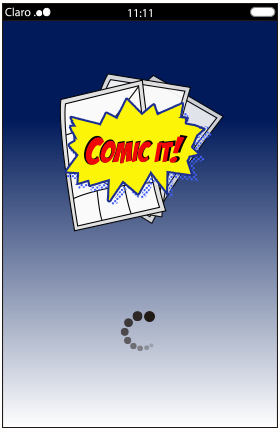
\includegraphics[width=0.19\textwidth]{demo/demo1.jpg}
		\endgroup
		\begingroup
			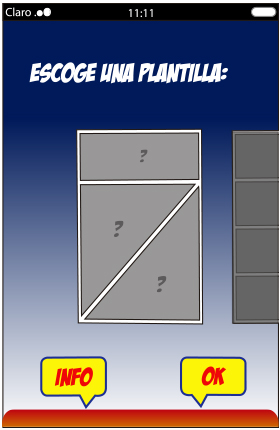
\includegraphics[width=0.19\textwidth]{demo/demo2.jpg}
		\endgroup
		\begingroup
			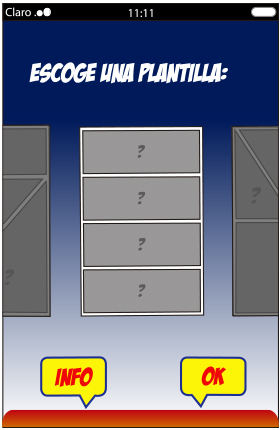
\includegraphics[width=0.19\textwidth]{demo/demo3.jpg}
		\endgroup
		\begingroup
			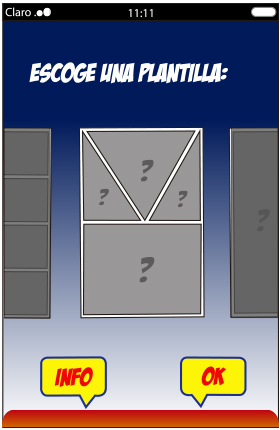
\includegraphics[width=0.19\textwidth]{demo/demo4.jpg}
		\endgroup
		\begingroup
			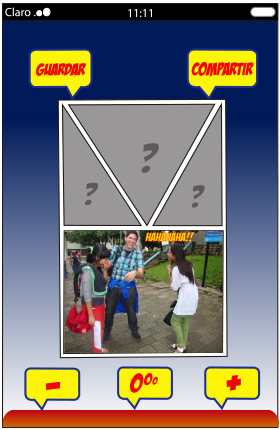
\includegraphics[width=0.19\textwidth]{demo/demo5.jpg}
		\endgroup
	\end{center}

Se observa la imagen inicial de la aplicación, seguido de las pantallas de selección de plantillas. Luego, puede verse un bosquejo de la aplicación en su parte más importante: La edición de la historieta.
 \newline
 \newline
En la parte superior, se tienen los botones 'Guardar' y 'Compartir'. Guardar, como su nombre lo indica, permitiría guardar la aplicación en la librería de imágenes del smartphone. 'Compartir' permitiría mostrar la historieta finalizada en las redes sociales, Twitter y Facebook.
 \newline
 \newline
En la parte inferior se observan los botones '-', '+' y el botón de selección de burbujas. Los dos primeros botones servirían para redimensionar las burbujas o íconos en pantalla.
           \newline
           \newline
	\begingroup
		\large{
			\textbf{
			           \newline
			           \newline
				Experiencias y Anécdotas: GitHub
				\newline
				\newline
			}
		}
	\endgroup
	\newline
	\newline	
	\begingroup
		\large{
			\textbf{
				Experiencias y Anécdotas: LaTeX
				\newline
				\newline
			}
		}
	\endgroup
	\textbf{Denny:\newline\newline} LaTeX es una buena herramienta para elaborar documentos. Muy útil bajo ciertas circunstancias, como la creación de libros (en especial de tipo matemáticos), pero bajo otras es probable que el usuario prefiera una herramienta de la categoría "WYSIWYG".
\newline
\newline
Aprender a elaborar un documento en LaTeX ha sido relativamente fácil, ya que hay muchos Websites en donde se especifica cómo utilizarlo, y sus comandos son hasta cierto punto intuitivos. Lo que no ha sido fácil, es lograr que el código se compile. Y es que la simple acción de identar el código, o dar saltos de linea,  podria hacer que el documento no se pueda compilar. A esto habría que agregarle, que los errores de compilación son difíciles de interpretar. 
\newline
\newline
LaTex tiene un potencial bastante bueno, en cuanto a la elaboración de documentos que, sin duda, se podría aprovechar muy bien con un poco más de práctica, como la inserción de ecuaciones en la redacción de un libro. Pero en cuanto a la elaboración de presentaciones, necesita un toque más multimedia, para poder satisfacer las necesidades de los usuarios.
\newline
\newline


\textbf{Liliana:\newline\newline}
\newline
\newline
\end{document}


